\documentclass[a4paper, oneside, final]{scrartcl} 
\usepackage{soul}
\usepackage{scrlayer-scrpage}
\usepackage{titlesec}
\usepackage{graphicx}
\usepackage{tabularx,colortbl}
\usepackage{multirow}
\usepackage{hyperref}
\usepackage{comment}
\titleformat{\section}{\small\scshape\raggedright}{}{0em}{}[\titlerule] 
\newcommand{\gray}{\rowcolor[gray]{.90}}
\usepackage{geometry}
\geometry{a4paper,right=20mm,left=20mm,top=20mm}

\begin{document}
	\fontsize{9px}{11px}\selectfont
	\pagestyle{empty} % non-numbered pages
	\begin{center} 
		%====================================================================================================
		%PERSONAL DATA_______________________________________________________________________________________
		%====================================================================================================
		\section{Dr. Silvia-Laura Pintea}
		\begin{tabular}{ll}
		    \begin{tabular}{l}
                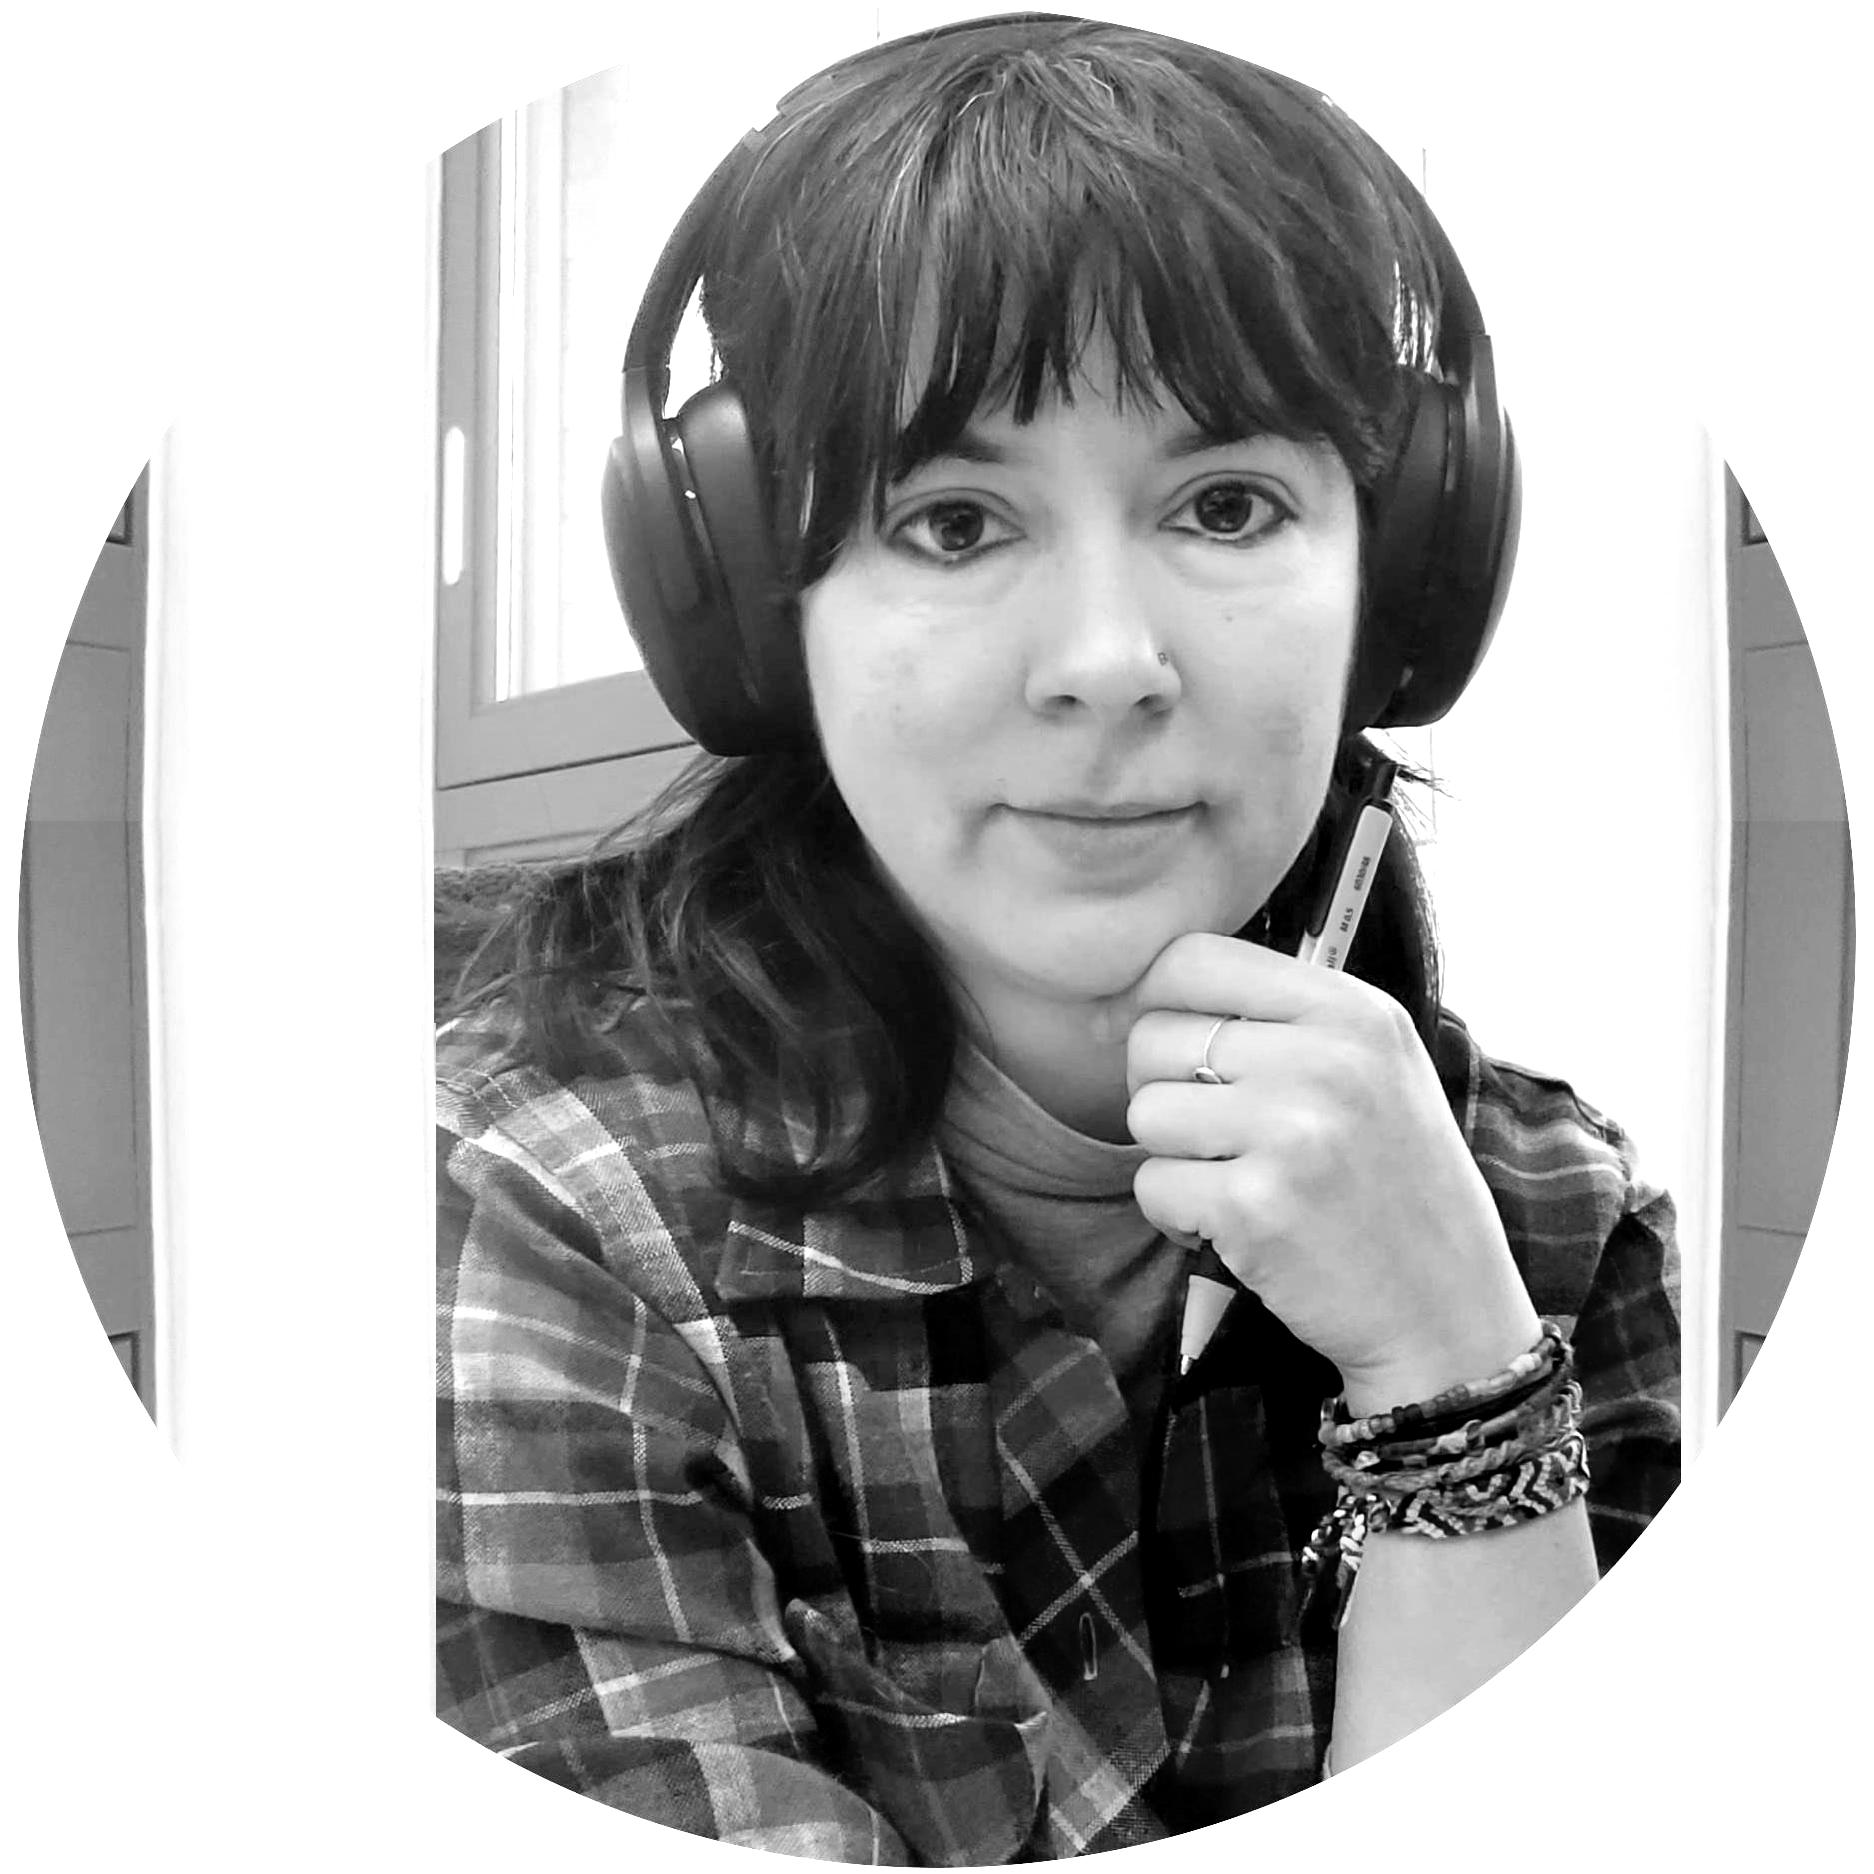
\includegraphics[width=3cm, height=3cm]{id}
		    \end{tabular}&
		    \begin{tabular}{l}
                   \textbf{\textsc{Computer Vision Researcher}}\\
                   \textsc{Nationality:} Dutch $\mid$ \textsc{Pronouns:} she\slash her\slash hers.\\
                   \textsc{Roles:} Researcher, lecturer, mentor, invited speaker, computer scientist.\\ 
                   \textsc{Email:} \href{mailto:silvia.laura.pintea@gmail.com}{Silvia[dot]Laura[dot]Pintea[at]gmail[dot]com}\\
                   \textsc{Webpage:} \href{https://silvialaurapintea.github.io}{http://silvialaurapintea.github.io} \vspace{5px}\\
                    My work is in the field of AI, specifically Computer Vision and Deep Learning, where \\
                    I have extensive experience with video and image analysis, specifically scale-invariance,\\
                    video motion representations and regression problems.\\
                    My current focus is on effective video analysis and robust motion representations.
		        \end{tabular}\\
            \end{tabular}
		%====================================================================================================
		%Work exps___________________________________________________________________________________________
		%====================================================================================================
		\section{Work Experience}
        \begin{tabular}{p{3.5cm}@{\hskip 0.3in}p{12.3cm}}
			%TiU_________________________________________________________________________
			\gray \textsc{\textbf{Assistant prof.}} & \textsc{\textbf{Department of Intelligent Systems (DIS), TiU, Tilburg, NL}}\\
			\textsc{Job Description}               & Physics priors for accurate and computationally efficient video and motion analysis.\\ 
			\textsc{Period}                        & \textsc{June 2025 --- Present} 
            \vspace{5px}\\
			%LKEB_________________________________________________________________________
			\gray \textsc{\textbf{Postdoc}} & \textsc{\textbf{Division of Image Processing (LKEB), LUMC, Leiden, NL}}\\
            \gray (Guest researcher)               & \textsc{\textbf{Vision Lab, Delft University of Technology (TUDelft), Delft, NL}}\\
			\textsc{Job Description}               & Efficient video and motion representations towards surgery video analysis.\\ 
			\textsc{Period}                        & \textsc{May 2022 --- April 2025} 
            \vspace{5px}\\
			%TUDelft_________________________________________________________________________
			\gray \textsc{\textbf{Researcher}} & \textsc{\textbf{Vision Lab, Delft University of Technology (TUDelft), Delft, NL}}\\
			\textsc{Job Description}            & Focus on Deep Learning scale-invariance and efficiency.\\
			\textsc{Period}                     & \textsc{July 2020 --- February 2022} 
            \vspace{5px}\\
			%TUDelft_________________________________________________________________________
			\gray \textsc{\textbf{Postdoc}}     & \textsc{\textbf{Vision Lab, Delft University of Technology (TUDelft), Delft, NL}}\\
			\textsc{Job Description}            & Collaboration with LUMC and the Geophysics department at TUDelft.
                                                Working on image and video analysis: geometric priors, scale-invariance, video representations, etc.\\
			\textsc{Period}                     & \textsc{July 2016 --- July 2020} 
            \vspace{5px}\\
			%Blippar________________________________________________________________________
            \gray \textsc{\textbf{R\&D Engineer}}   & \textsc{\textbf{Layar\slash Blippar, Amsterdam, NL} (augmented reality company)}\\
            \textsc{Job Description}                & Focus on efficient large-scale image matching and retrieval, using C${++}$.\\
			\textsc{Period}                         & \textsc{January --- June 2016} 
			%Blippar________________________________________________________________________
		\end{tabular}
		%====================================================================================================
		%EDUCATION___________________________________________________________________________________________
		%====================================================================================================
		\section{Education}
        \begin{tabular}{p{3.5cm}@{\hskip 0.3in}p{12.3cm}}
			%PHD__________________________________________________________________________________
			\gray \textsc{\textbf{PhD}}     & \textbf{\textsc{Computer Vision}}, University of Amsterdam (UvA), Amsterdam, NL\\
			\textsc{Focus}                  & Motion prediction, object localization, video representation learning \\
			\textsc{Thesis Title}           & {\href{http://dare.uva.nl/search?identifier=90ad88f5-c16e-4450-86f2-23faa250fcab}{Continuous Learning in Computer Vision}}\\
            \textsc{Period}                 & \textsc{2011 -- 2015}
            \vspace{5px}\\
			%MASTER______________________________________________________________________________
			\gray \textsc{\textbf{MSc}}         & \textbf{\textsc{Artificial Intelligence}}, University of Amsterdam, (UvA) Amsterdam, NL\\
			\textsc{Focus}                      & Machine Learning, Computer Vision, Neural Networks, Game Theory.\\
            \textsc{Period} $\mid$ \textsc{Avg. Grade}   & \textsc{2009  -- 2011} $|$ 8.31 (out of 10)
            \vspace{5px}\\
			%BACHELORS______________________________________________________________________________
			\gray \textsc{\textbf{BSc}}         & \textbf{\textsc{Computer Science}}, University of Bucharest, Faculty of Mathematics and Computer Science, Bucharest, RO\\
			\textsc{Focus}                      & Algorithms and data structures, Object oriented programming, Formal methods.\\ 
            \textsc{Period} $\mid$ \textsc{Avg. grade}   & \textsc{2005 -- 2008} $|$ 9.40 (out of 10)
		\end{tabular}

		%====================================================================================================
		%TEACHING____________________________________________________________________________________________
		%====================================================================================================
		\section{Teaching and guiding}
        \begin{tabular}{p{3.5cm}@{\hskip 0.3in}p{12.3cm}}
			%Teaching___________________________________________________________________________________
			\textsc{Teaching}		            & BSc Introduction to deep learning (TiU, 2025-2026), BSc Computer vision (TiU, 2025-2026), MSc Image analysis (TiU, 2025-2026)\\
                                                & BSc Image processing (TUDelft, 2018-2022), MSc Computer vision by deep learning (TUDelft, 2018-2022)\\
			\textsc{PhD copromotor}             & Dr. Yancong Lin, Dr. Xin Liu\\ 
			\textsc{PhD adviser}                & Xiaotong Zhang, Faeze Gholamiankhah, Xin Liu, Yancong Lin, Vedran Vukotic (visting student), Abolfazi Nadi (visiting student)\\ 
			\textsc{MSc adviser}                & Tobias Stahl, Yichao Zhang, Chengqiu Zhang, Xilin Li, Yue Liu, Omar Hommos, Xiaoming Wen, Jian Zheng, Ziyu Bao, Yordan Dimitrov, Nikhil Saldanha, Ziyu Bao, Jimmy Vlekke, Frans de Boer, Douwe Hoonhout\\
		\end{tabular}

		%====================================================================================================
		%Qualification_______________________________________________________________________________________
		%====================================================================================================
		\section{Qualifications and training}
        \begin{tabular}{p{3.5cm}@{\hskip 0.3in}p{12.3cm}}
			%LANGUAGES___________________________________________________________________________________
            \textsc{BKO}                   & University teaching qualifications (TUDelft), completed in 2022.\\
            \textsc{PDP}                   & Tenure Track Personal Development Program (TUDelft), completed in 2021.\\
		\end{tabular}

		%====================================================================================================
		\section{Community service, awards \& other}
        \begin{tabular}{p{4.5cm}@{\hskip 0.3in}p{11.3cm}}
			%Other___________________________________________________________________________________
            \textsc{Invited speaker}            & Digital Society Institute Meet Up (Twente, 2026), Startup Village (Amsterdam, 2022), AIRLab (Delft, 2019), NucTech meeting (Delft, 2018), Delft-Leiden Deep Learning Seminars (Leiden, 2019)\\
            \textsc{Invited lecturer}           & Deep Learning MSc course TUDelft (2019)\\
            \textsc{Award}                      & Outstanding Reviewer: CVPR (2025, 2022, 2021), ICCV (2021), ECCV (2022), BMVC(2022, 2021)\\ 
                                                & Best paper award for the Workshop on Hands, ECCVw (2018)\\  
            \textsc{International conferences}  & ICPR (2026), ICCV (2023,2021), CVPR (2021), ECCV (2020, 2016, 2014), ICIP (2018, 2016)\\
            \textsc{Local conferences\slash events} &  NCCV (2018 - 2023, 2026), Video Understanding Symposium (2023), NVPHBV (2017), ICT.Open (2016, 2012)\\
            \textsc{Reviewer (since 2012)}      & CVPR, ECCV/ICCV, BMVC, WACV, ICPR, TIP, IJCV\\
			\textsc{Programming}                & Python, PyTorch, Jax, TensorFlow, C\slash C++, Caffe, Torch, PHP,\\ 
			                                    & Java, OpenCV, Dlib, Shogun, LibSVM, VlFeat, Yael, Matlab\\
		\end{tabular}
		%====================================================================================================
		
        %====================================================================================================
		%Publications________________________________________________________________________________________
		%====================================================================================================
		\section{Key publications}
        \begin{tabular}{p{16.7cm}}
        \begin{flushleft}
            \vspace{-10px}
            \begin{itemize}
                \item \textsc{\textbf{\href{https://github.com/SilviaLauraPintea/video_approx}{``Deep kernel video approximation for unsupervised action segmentation"}}} \emph{SL Pintea}, J. Dijkstra, International Conference on Pattern Recognition (ICPR) 2026.\\[3px]
			%  ________________________________________________________________________________
                
                \item \textsc{\textbf{\href{https://github.com/SilviaLauraPintea/reg-cls}{``A step towards understanding why classification helps regression"}}} \emph{SL Pintea}, Y. Lin, J. Dijkstra, JC van Gemert, International Conference on Computer Vision (ICCV) 2023.\\[3px]
			%  ________________________________________________________________________________

                \item \textsc{\textbf{\href{https://github.com/SilviaLauraPintea/N-JetNet}{``Resolution learning in deep convolutional networks using scale-space theory"}}}, \emph{SL Pintea}, N Tomen, SF Goes, M Loog, JC van Gemert, Transactions on Image Processing (TIP), 2021.\\[3px]
			%  ________________________________________________________________________________
                \item \textsc{\textbf{``No frame left behind: Full Video Action Recognition"}}, X Liu, \emph{SL Pintea}, FK Nejadasl, O Booij, JC van Gemert. Computer Vision and Pattern Recognition (CVPR), 2021.\\[3px]
                
			%  ________________________________________________________________________________
                \item \textsc{\textbf{\href{https://github.com/SilviaLauraPintea/acceleration-magnification.github.io}{``Video Acceleration Magnification"}}}, Y Zhang, \emph{SL Pintea}, Jan C. van Gemert, Computer Vision and Pattern Recognition (CVPR), 2017.\\[3px]
			%  ________________________________________________________________________________
        \item \textsc{\textbf{\href{http://github.com/SilviaLauraPintea/DejaVu}{``D\'{e}j\`{a} Vu: Motion Prediction in Static Images."}}}, \emph{SL Pintea}, JC van Gemert, AWM Smeulders, European Conference on Computer Vision (ECCV), 2014.\\[10px]
            \end{itemize}
            \vspace{5px}
        \textsc{\textbf{Complete list of publications:}} \href{https://scholar.google.nl/citations?user=shTkx9EAAAAJ&hl=en}{https://scholar.google.nl/citations?user=shTkx9EAAAAJ\&hl=en}\\
        \end{flushleft}
		\end{tabular}
        %====================================================================================================
		%\section{References}
        %\begin{tabular}{p{3.5cm}@{\hskip 0.3in}p{12.3cm}}
	    	%References___________________________________________________________________________________
            %Assistant Prof. UvA     & Dr. Pascal Mettes \href{mailto:P.S.M.Mettes@uva.nl}{(P[dot]S[dot]M[dot]Mettes[at]uva[dot]nl)} \\
            %Assistant Prof. TUDelft & Dr. Nergis Tomen \href{mailto:n.tomen@tudelft.nl}{N[dot]Tomen[at]tudelft[dot]nl} \\
            %Associate Prof. TUDelft & Dr. Jan van Gemeert \href{mailto:J.C.vanGemert@tudelft.nl}{(J[dot]C[dot]vanGemert[at]tudelft[dot]nl)} \\
            %Prof. LUMC \& TUDelft   & Prof. Dr. Boudewijn P.F. Lelieveldt \href{mailto:b.p.f.lelieveldt@lumc.nl}{(B[dot]P[dot]F[dot]Lelieveldt[at]lumc[dot]nl)}\\
	        %RU \& TUDelft      & \href{mailto:marco.loog@ru.nl}{Prof. Dr. Marco Loog (Marco[dot]Loog[at]ru[dot]nl)}\\
			%\multicolumn{2}{c}{}\\
		%\end{tabular}
	\end{center}
\end{document}

